\documentclass[11pt,a4paper]{article}
\usepackage[margin=23mm]{geometry}
\usepackage{graphicx,booktabs,hyperref}
\hypersetup{hidelinks}
\setlength{\parindent}{0pt}
\setlength{\parskip}{.55em}
\title{Recognising a distorted recording among 105,705 tracks}
\author{Felix Lund Frandsen \and Nikolaos Iliakis \and Krzysztof Kisiel \and Konstantinos Tzimoulias}
\date{24 November 2026}
\begin{document}
\maketitle
A listener wants the title of a song playing underneath speech. Each extra song in the catalogue adds another plausible wrong answer, and checking every recording costs time. We ask how well a short excerpt identifies its source and how much search we can skip as the catalogue grows. We train a fingerprint, compare two course algorithms against exhaustive search, and examine a wrong answer where the two track IDs contain identical audio.

\section*{What makes ten seconds recognisable?}
We use the \href{https://github.com/mdeff/fma}{Free Music Archive (FMA)}. We decode excerpts to 24 kHz mono, take ten-second windows every five seconds, and discard near-silent reference windows. Medium supplies 110,320 searchable windows from 24,970 tracks. Large supplies 464,464 from 105,705 tracks. We preserve the Medium windows and add 80,735 tracks, so a change in recognition on the same queries measures the effect of additional competitors. Small has its own released head and query draws; we use it separately to investigate recording identity.

Our independently studied method is neural audio fingerprinting, adapted from \href{https://arxiv.org/abs/2511.05399}{Singh et al.} A frozen MuQ encoder represents each window with 1,024 features. We train a projection head on clean and distorted versions of the same passage. The training objective pulls these pairs together and separates examples from other recordings. The output is a 256-dimensional unit vector, so the dot product measures cosine similarity. Training and evaluation draw from different track IDs. Voice-over training and testing use different LibriSpeech speakers. TikTok-like queries are synthetic speed, speech and compression effects.

Does training the head buy anything if search is already exact? On 8,992 held-out Medium TikTok-like clips, exhaustive search identified 5,217 with raw MuQ features (58.02\%) and 8,411 with the trained fingerprint (93.54\%). Of the changes, 3,219 corrected a previous mistake and 25 introduced one. The net gain was 35.52 percentage points (95\% paired song-bootstrap interval 34.52--36.56). This compares the complete projection, including the change in dimension. It justifies keeping the head fixed when testing indexes.

\section*{How much of the catalogue must we search?}
Exhaustive lookup returns the track of the reference window with the highest cosine. Angular locality-sensitive hashing (LSH) uses random hyperplanes to place similar windows into common buckets. We score candidates drawn from several tables and nearby buckets. Longer hash keys were faster but missed distorted recordings. After seeing the first Medium comparison we explored the best standard-development accuracy setting: ten bits, 64 tables and three extra probes. We froze it for the catalogue comparison. The setting choice on Medium was exploratory.

Spherical k-means learns partitions from the reference vectors. An inverted-file index (IVF) stores each centroid's windows together. We fit 256 unit centroids and visit the nearest 16 lists per query. Both indexes approximate the same exhaustive score, but their candidates come from different partitions.

\begin{center}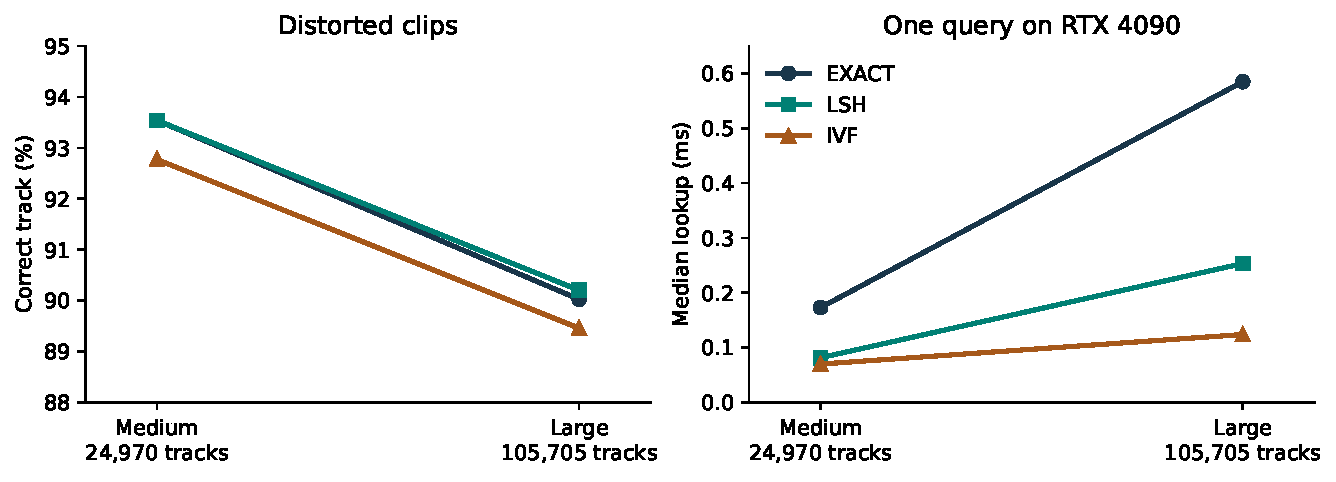
\includegraphics[width=.94\linewidth]{figures/report-catalogues.pdf}\end{center}
{\small Figure 1. The same 8,992 TikTok-like clips are searched against both catalogues. The right panel uses the original interleaved benchmark of 192 single queries on an RTX 4090 with the indexes resident in GPU memory. It times the lookup from a fingerprint.}

Adding Large's tracks reduced exhaustive recognition from 8,411 to 8,095 of 8,992 TikTok-like clips, and from 7,315 to 7,185 of 7,458 standard clips. No previously wrong exhaustive answer became correct in these paired comparisons. On Large, LSH identified 90.20\% of TikTok-like clips, exhaustive search 90.02\%, and IVF 89.46\%. A highest-cosine neighbour can have the wrong track ID; an approximate search can sometimes skip it. The small LSH lead is specific to these clips.

For one Large lookup the original medians were 0.585 ms for exhaustive search, 0.253 ms for LSH and 0.124 ms for IVF. LSH therefore gave a $2.31\times$ lookup speedup while retaining recognition accuracy. For batches of 128, exhaustive search reached 95,267 queries/s, ahead of IVF at 89,420 and LSH at 7,057. Batching makes the dense matrix multiplication effective. The release rerun reproduced every accuracy count and the same ordering of methods on single and batched lookups.

\section*{When is a wrong ID the right recording?}
On Small we also ran the team's DBSCAN on windows with cosine similarity at least 0.9 and a minimum of two neighbours including the window itself. It labelled 82.6\% of windows as noise and linked 69 track pairs through shared clusters. A link suggests where to inspect the audio. For a distorted query from 11.28 s into track 086761, exhaustive search returned a window at 10 s in track 074348. Both are Marco Trovatello's \emph{Be Sweet}. The decoded 24 kHz mono samples have identical SHA-256 digests, and all five released reference fingerprints match. Strict ID scoring records a miss, although the listener would see the same artist and title. One verified pair does not establish the identity of every linked pair.

For interactive lookup on this GPU, LSH gave near-exhaustive identification; IVF was fastest when some loss in recognition was acceptable. For bulk queries exhaustive search was fastest on Large. These conclusions cover ten-second synthetic queries drawn from the Medium query pool. Detecting songs absent from the collection and recognising real microphone captures are distinct evaluation problems. The notebook reports the measured trade-offs; a paired phone test remains open.
\end{document}
